%----------------------------------------------------------------------------------------
%    PACKAGES AND THEMES
%----------------------------------------------------------------------------------------

\documentclass[aspectratio=169,12.5pt,xcolor=dvipsnames]{beamer}
\usetheme{SimpleDarkBlue}

\usepackage{hyperref}
\usepackage{graphicx} % Allows including images
\usepackage{booktabs} % Allows the use of \toprule, \midrule and \bottomrule in tables
\usepackage{caption}
\usepackage{amsmath}
\usepackage{tikz}
\usepackage{nicematrix}

%----------------------------------------------------------Alguns setups
%----------------------------------------------------------

%----------------------------------------------------------------------------------------
%    TITLE PAGE
%----------------------------------------------------------------------------------------

\title{Relatório primeira prática}
\subtitle{Elétron : partícula (razão de sua carga e massa) : onda (difração Debye-Scherrer polycrystalline lattice)}

\author{João Vítor Lima de Oliveira
\\
Guilherme Aranha}

\institute
{
    Instituto de Física de São Carlos
    \\
    Universidade de São Paulo % Your institution for the title page
}
\date{\today} % Date, can be changed to a custom date

%----------------------------------------------------------------------------------------
%    PRESENTATION SLIDES
%----------------------------------------------------------------------------------------

\begin{document}

\begin{frame}
    % Print the title page as the first slide
    \titlepage
\end{frame}

\begin{frame}{Sumário}
    % Throughout your presentation, if you choose to use \section{} and \subsection{} commands, these will automatically be printed on this slide as an overview of your presentation
    \tableofcontents
\end{frame}

%------------------------------------------------
\section{Motivação}
%------------------------------------------------

\begin{frame}{Motivação}
    \Huge{\centerline{\textbf{Motivação}}}
\end{frame}

\begin{frame}{Linha do tempo}

        \begin{center}
        \begin{figure}
        \caption{Linha do tempo dos experimentos que antecederam a formulação da hipótese de Broglie, e que podem tê-lo influenciado.}
        \vspace*{-0.25cm}
        \includegraphics[width=0.75\textwidth,height=0.70\textheight,keepaspectratio]{figuras/linha o tempo.png}\par
        {\scriptsize Fonte: Elaborado pelo autor.}
        \end{figure}
        \end{center}
    
\end{frame}


\begin{frame}{Linha do tempo}
\centering
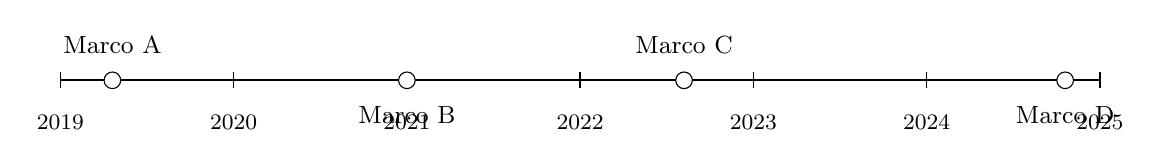
\begin{tikzpicture}[x=2.2cm, y=1cm, >=stealth,
    event/.style={circle, draw, fill=white, inner sep=1.5pt, minimum size=6pt},
    label above/.style={font=\small, align=center, above=6pt},
    label below/.style={font=\small, align=center, below=6pt}
]
  \draw[line width=0.6pt] (0,0) -- (6,0);
  \foreach \x/\txt in {0/2019,1/2020,2/2021,3/2022,4/2023,5/2024,6/2025}{
    \draw[line width=0.6pt] (\x,0.1) -- (\x,-0.1) node[below=6pt,font=\footnotesize] {\txt};
  }

  \node[event] (e1) at (0.3,0) {}; \node[label above] at (e1) {Marco A};
  \node[event] (e2) at (2.0,0) {}; \node[label below] at (e2) {Marco B};
  \node[event] (e3) at (3.6,0) {}; \node[label above] at (e3) {Marco C};
  \node[event] (e4) at (5.8,0) {}; \node[label below] at (e4) {Marco D};
\end{tikzpicture}
\end{frame}


\begin{frame}{Dualidade Onda-Partícula para Luz}

    \begin{columns}[c]
        \column{.45\textwidth}
        \begin{figure}
          \centering
          \caption{Albert Einstein}
          \includegraphics[width=4.25cm]{figuras/albert.png}\par
          {\scriptsize Fonte: Retirado da internet.}
        \end{figure}

        \column{.45\textwidth}
        Em \textbf{1905}, Albert Einstein apresenta o conceito de dualidade onda-partícula para a \textbf{luz} de forma a explicar o efeito fotoelétrico.

    \end{columns}

    
\end{frame}

%------------------------------------------------

\begin{frame}{Dualidade Onda-Partícula para Matéria}

    \begin{columns}[c]

        \column{.45\textwidth}
        \begin{figure}
          \centering
          \caption{Louis de Broglie}
          \includegraphics[width=4.25cm]{figuras/Prince_Louis-Victor_de_Broglie.jpg}\par
          {\scriptsize Fonte: Retirado da internet.}
        \end{figure}

        \column{.45\textwidth}
        Em \textbf{1924}, Louis de Broglie, em sua tese de doutorado, expande o conceito de dualidade onda-partícula para toda \textbf{matéria}.

    \end{columns}

\end{frame}

%------------------------------------------------
\section{Objetivos}
%------------------------------------------------
\begin{frame}{Objetivos}
    \Huge{\centerline{\textbf{Objetivos}}}
\end{frame}

\begin{frame}{Objetivos}

\vspace{1\baselineskip}

    \begin{itemize}
        \item Estudar comportamento ondulatório da matéria
        
        \item Comparar os comprimentos de onda de de Broglie com aqueles previstos pela lei de Bragg
        
        \item Determinar a constante de Planck
        
        \item Encontrar as distâncias interplanares do cristal de grafite utilizado no experimento
    \end{itemize}
\end{frame}
%------------------------------------------------
\section{Metodologia}

%------------------------------------------------

\begin{frame}{Comprimento de onda de de Broglie}

    de Broglie relaciona o momento de uma partícula $p$, a constante de Planck $h$ e seu comprimento de onda $\lambda$.        
    \begin{equation}
        \lambda = \frac{h}{p}
    \end{equation}

\end{frame}

%------------------------------------------------
\begin{frame}{Metodologia}
    \Huge{\centerline{\textbf{Metodologia}}}
\end{frame}

\begin{frame}{Comparação do comprimento de onda de Bragg e de Broglie}

Queremos comparar o comprimento de onda dos raios X utilizados por Bragg em seus experimentos de difração de cristais com o comprimento de onda de elétrons acelerados a alguns quilovolts, segundo a hipótese de de Broglie, para verificar se a teoria desenvolvida por Bragg é aplicável a esse problema.

\begin{equation}
\begin{aligned}
\lambda &= \frac{h}{p} = \frac{h}{\sqrt{2 m_e e V}} \\[6pt]
        &= \frac{6.63 \times 10^{-34}}
        {\sqrt{2 (9.11 \times 10^{-31})(1.6 \times 10^{-19})(5 \times 10^3)}} \\[6pt]
        &\approx 1.74 \times 10^{-11} \ \text{m}
\end{aligned}
\end{equation}
\end{frame}

\begin{frame}{Difração de DEBYE-SCHERRER}

        \begin{center}
        \begin{figure}
        \caption{Representação do método de difração Debye-Scherrer.}
        \vspace*{-0.25cm}
        \includegraphics[width=0.75\textwidth,height=0.75\textheight,keepaspectratio]{figuras/debye.png}\par
        {\scriptsize Fonte: Adaptado da Wikipedia.}
        \end{figure}
        \end{center}
    
\end{frame}



\begin{frame}{Diferença entre um policristal e um mono cristal.}

    \begin{columns}[c]
      

        \column{.45\textwidth}
        \begin{figure}
          \centering
          \caption{Representação da estrutura de mono cristais e policristais.}
          \includegraphics[width=4.10cm]{figuras/poli_mono2.png}\par
          {\scriptsize Fonte: Retirado da internet.}
        \end{figure}

  \column{.45\textwidth}
        Os policristais são sólidos formados por muitos pequenos monocristais com diferentes
orientações.

    \end{columns}

    
\end{frame}

\begin{frame}

        \begin{center}
        \begin{figure}
          \caption{Representação da estrutura de diferentes tipos de cristais.}
        % \vspace*{-0.45cm}
        \includegraphics[width=0.75\textwidth,height=0.75\textheight,keepaspectratio]{figuras/poli_mono.jpg}\par
          {\scriptsize Fonte: Retirado da internet.}
        \end{figure}
        \end{center}



    
\end{frame}

\begin{frame}{Policristal de grafite.}

        \begin{center}
        \begin{figure}
        \caption{Exemplo de estrutura de um policristal de grafite.}
        \vspace*{-0.25cm}
        \includegraphics[width=0.75\textwidth,height=0.75\textheight,keepaspectratio]{figuras/Crystallographic-structure-of-graphite.png}\par
        {\scriptsize Fonte: Retirado de \cite{STEFANESCU2016102}.}
        \end{figure}
        \end{center}
    
\end{frame}


\begin{frame}{Equipamento utilizado}

    \begin{columns}[c]
        \column{.45\textwidth}
        \begin{figure}
          \centering
          \caption{Equipamento utilizado (visão frontal).}
          \includegraphics[width=4.25cm]{figuras/metodologia_3.jpeg}\par
          {\scriptsize Fonte: Elaborado pelo autor.}
        \end{figure}

        \column{.45\textwidth}
        \begin{figure}
          \centering
          \caption{Equipamento utilizado (visão lateral).}
          \includegraphics[width=4.25cm]{figuras/metodologia_2.jpeg}\par
          {\scriptsize Fonte: Elaborado pelo autor.}
        \end{figure}

    \end{columns}

    
\end{frame}


\begin{frame}{Difração}

    \begin{columns}[c]
        \column{.45\textwidth}
        \begin{figure}
          \centering
          \caption{Padão de difração observado.}
          \includegraphics[width=4.25cm]{figuras/metodologia_1.jpeg}\par
        {\scriptsize Fonte: Elabora pelo autor.}
        \end{figure}

        \column{.45\textwidth}
        Padrão de difração observado.
    \end{columns}

    
\end{frame}

%------------------------------------------------
\section{Resultados}
%------------------------------------------------

\begin{frame}{Resultados}
    \Huge{\centerline{\textbf{Resultados}}}
\end{frame}


\begin{frame}{Resultados}

        \begin{center}
        \begin{figure}
        \caption{Dados experimentais obtidos, curva Diametros [cm] $\times$ $V$ (Tensão) em [Volts], do primeiro padrão de Difração.}
        \vspace*{-0.25cm}
        \includegraphics[width=0.75\textwidth,height=0.75\textheight,keepaspectratio]{figuras/fit1.png}\par
        {\scriptsize Fonte: Elabora pelo autor.}
        \end{figure}
        \end{center}
    
\end{frame}

\begin{frame}{Resultados}

        \begin{center}
        \begin{figure}
        \caption{Dados experimentais obtidos, curva Diametros [cm] $\times$ $V$ (Tensão) em [Volts], do segundo padrão de Difração.}
        \vspace*{-0.25cm}
        \includegraphics[width=0.75\textwidth,height=0.75\textheight,keepaspectratio]{figuras/fit2.png}\par
        % {\scriptsize Fonte: Elabora pelo autor.}
        \end{figure}
        \end{center}
    
\end{frame}

\begin{frame}{Equação utilizada no ajuste de curva}
    
    Equação utilizada no ajuste de curva para os dados experimentais obtidos, curva Diametros [cm] $\times$ $V$ (Tensão) em [Volts], do primeiro e segundo padrão de Difração
    \begin{equation}
    r = \frac{l}{2d} \frac{h}{\sqrt{2 m e V}}
    \end{equation}

    onde usamos, para realizar o ajuste númerico,
    \begin{equation}
    r = \alpha V^{-1/2}
    \end{equation}

\end{frame}

\begin{frame}{Funcionamento do código utilizado na analise dos dados}

\centering
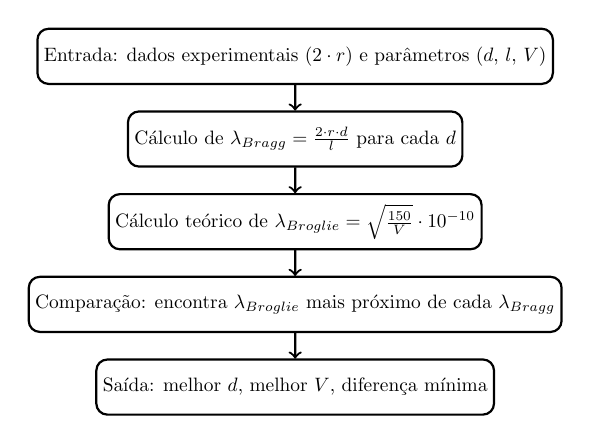
\begin{tikzpicture}[node distance=1.5cm, auto, thick, scale=0.7, every node/.style={scale=0.7}]
\tikzstyle{block} = [rectangle, draw, rounded corners, text centered, minimum width=5cm, minimum height=1cm]

\node[block] (entrada) {Entrada: dados experimentais ($2\cdot r$) e parâmetros ($d$, $l$, $V$)};
\node[block, below of=entrada] (calc1) {Cálculo de $\lambda_{Bragg} = \tfrac{2\cdot r \cdot d}{l}$ para cada $d$};
\node[block, below of=calc1] (calc2) {Cálculo teórico de $\lambda_{Broglie} = \sqrt{\tfrac{150}{V}} \cdot 10^{-10}$};
\node[block, below of=calc2] (comp) {Comparação: encontra $\lambda_{Broglie}$ mais próximo de cada $\lambda_{Bragg}$};
\node[block, below of=comp] (saida) {Saída: melhor $d$, melhor $V$, diferença mínima};

\draw[->] (entrada) -- (calc1);
\draw[->] (calc1) -- (calc2);
\draw[->] (calc2) -- (comp);
\draw[->] (comp) -- (saida);

\end{tikzpicture}

\vspace{0.5cm}
\textbf{Resumo:} O código busca a correspondência entre teoria ($\lambda_{Broglie}$) e experimento ($\lambda_{Bragg}$), 
determinando a melhor voltagem e distância interplanar para cada medida.


\end{frame}

%------------------------------------------------


\begin{frame}{Resultados}

        \begin{center}
        \begin{figure}
        \caption{Comparação entre $\lambda_{Broglie}$ e $\lambda_{Bragg}$ (normalizados)}
        \vspace*{-0.25cm}
        \includegraphics[width=0.75\textwidth,height=0.75\textheight,keepaspectratio]{figuras/plot1.png}\par
        % {\scriptsize Fonte: Elabora pelo autor.}
        \end{figure}
        \end{center}
    
\end{frame}

\begin{frame}{Resultados}

        \begin{center}
        \begin{figure}
        \caption{Diferença entre $\lambda_{Bragg}$ e $\lambda_{Broglie}$ (normalizados)}
        \vspace*{-0.25cm}
        \includegraphics[width=0.75\textwidth,height=0.75\textheight,keepaspectratio]{figuras/plot3.png}\par
        % {\scriptsize Fonte: Elabora pelo autor.}
        \end{figure}
        \end{center}
    
\end{frame}

\begin{frame}{Distâncias
interplanares do policristal de grafite}

    \begin{table}[h!]
    \centering
    \scalebox{1.50}{
    \begin{tabular}{c c}
    \hline
    Índice & \(d \, (\text{\AA})\) \\
    \hline
    1 & 2.130 \\
    2 & 1.230 \\
    3 & 0.805 \\
    4 & 0.591 \\
    5 & 0.465 \\
    \hline
    \end{tabular}}
    \caption{Valores $d$ (distâncias
interplanares) em ångströms (\AA)}
    \end{table}
    


\end{frame}

\begin{frame}{Distâncias
interplanares associadas ao comprimento de onda de Bragg}

    \begin{table}[h!]
    \centering
    \scalebox{0.90}{
    \begin{tabular}{c c c}
    \hline
    Medida & $\lambda_{Bragg}$ (\AA) & $d$ (\AA) \\
    \hline
    0  & $0.1806$ & $0.4650$ \\
    1  & $0.1806$ & $0.4650$ \\
    2  & $0.2100$ & $0.5910$ \\
    3  & $0.2041$ & $0.5910$ \\
    4  & $0.1987$ & $0.5910$ \\
    5  & $0.1936$ & $0.5910$ \\
    6  & $0.1890$ & $0.5910$ \\
    7  & $0.1768$ & $0.5910$ \\
    8  & $0.1732$ & $0.5910$ \\
    9  & $0.1732$ & $0.5910$ \\
    10 & $0.2236$ & $0.8050$ \\
    11 & $0.2236$ & $0.8050$ \\
    12 & $0.2165$ & $0.8050$ \\
    13 & $0.2100$ & $0.8050$ \\
    \hline
    \end{tabular}}
    \caption{Valores de $\lambda_{Bragg}$ e $d$ (distâncias
interplanares), ambos em ångströms (\AA), para cada medida.}
    \end{table}
    

\end{frame}


\begin{frame}{Resultados}

        \begin{center}
        \begin{figure}
        \caption{Curva $\lambda_{Broglie}$ (valores melhor ajustados) $\times$ $\frac{1}{\sqrt{V}}$}
        \vspace*{-0.25cm}
        \includegraphics[width=0.75\textwidth,height=0.75\textheight,keepaspectratio]{figuras/fit3.png}\par
        % {\scriptsize Fonte: Elabora pelo autor.}
        \end{figure}
        \end{center}
    
\end{frame}

\begin{frame}{Econtrando o valor de $h$}

Encontraremos o valor de $h$ a partir do ajuste dos dados experimentais, temos:
\begin{equation}
\lambda_{Broglie} = \frac{h}{\sqrt{2 m e}} \, V^{-\tfrac{1}{2}} = \alpha \cdot V^{-\tfrac{1}{2}}
\end{equation}
\indent Isso posto,

\begin{equation}
\alpha := \frac{h}{\beta} \quad ; \quad \beta := \sqrt{2 m e}
\end{equation}
\indent Dessa forma, isolando $h$, temos:
\begin{equation}
h = \alpha \cdot \beta
\end{equation}
com os valores de $\alpha = 1.224744 \times 10^{-09}$ $\pm 5.1885 \times 10^{-25}
$ e $\beta = 5.402747 \times 10^{-25}$ conhecidos, podemos encontrar $h$.

\begin{equation}
        h =  6.616988 \times 10^{-34} \pm 5.1885 \times 10^{-25} \text{[J$\cdot$s]}
\end{equation}

\end{frame}


%------------------------------------------------

\begin{frame}{Bibleografia}
    \footnotesize
    \bibliography{reference.bib}
    \bibliographystyle{apalike}
\end{frame}

%------------------------------------------------

\begin{frame}
    \Huge{\centerline{\textbf{Obrigado!}}}
\end{frame}

%----------------------------------------------------------------------------------------

\end{document}